\documentclass[unknownkeysallowed]{beamer}
\usepackage[utf8]{inputenc}
\usepackage[french,english]{babel}
\usepackage{../sty/beamer_js}
\usepackage{../sty/shortcuts_js}

\definecolor{tomcolor}{rgb}{0.,.3,.6}



\definecolor{kw}{RGB}{0,112,26}
\definecolor{var}{RGB}{0,133,182}
\definecolor{func}{RGB}{0,35,126}
\definecolor{palegreen}{RGB}{236,240,241}
\setbeamercolor{bgcolor}{fg=black!60,bg=palegreen}

\lstset{basicstyle=\color{tomcolor}\scriptsize\ttfamily}
\addbibresource{../biblio/biblio.bib}
\captionsetup[subfigure]{labelformat=empty}
\begin{document}

%%%%%%%%%%%%%%%%%%%%%%%%%%%%%%%%%%%%%%%%%%%%%%%%%%%%%%%%%%%%%%%%%%%%%%%%%%%%%%%
%%%%%%%%%%%%%%%%%%%%%%             Headers               %%%%%%%%%%%%%%%%%%%%%%
%%%%%%%%%%%%%%%%%%%%%%%%%%%%%%%%%%%%%%%%%%%%%%%%%%%%%%%%%%%%%%%%%%%%%%%%%%%%%%%


%%%%%%%%%%%%%%%%%%%%%%%%%%%%%%%%%%%%%%%%%%%%%%%%%%%%%%%%%%%%%%%%%%%%%%%%%%%%%%%
\begin{frame}
\bigskip
\bigskip
\begin{center}{
\LARGE\color{marron}
\textbf{\texttt{benchopt}:\\
		Benchmarking optimization Algorithms}
\textbf{ }\\
\vspace{0.5cm}
}

\color{marron}
% \textbf{or... an introduction to Beamer instead}
\end{center}

\vspace{0.5cm}

\begin{center}
\textbf{Thomas Moreau} \\
\vspace{0.1cm}
\url{http://tommoral.github.io}\\
\vspace{0.5cm}
INRIA - Parietal \\
\end{center}

\centering

\includegraphics[width=0.26\textwidth]{logo_inria}

\includegraphics[width=0.36\textwidth]{logo_parietal}

\end{frame}
%%%%%%%%%%%%%%%%%%%%%%%%%%%%%%%%%%%%%%%%%%%%%%%%%%%%%%%%%%%%%%%%%%%%%%%%%%%%%%%


%%%%%%%%%%%%%%%%%%%%%%%%%%%%%%%%%%%%%%%%%%%%%%%%%%%%%%%%%%%%%%%%%%%%%%%%%%%%%%%
\begin{frame}[fragile]{The problem}

    \begin{columns}
        \column{.5\textwidth}
        
\includegraphics[width=\textwidth]{tweet_steinner}
        
\includegraphics[width=\textwidth]{tweet_steinner2}
        \column{.5\textwidth}
            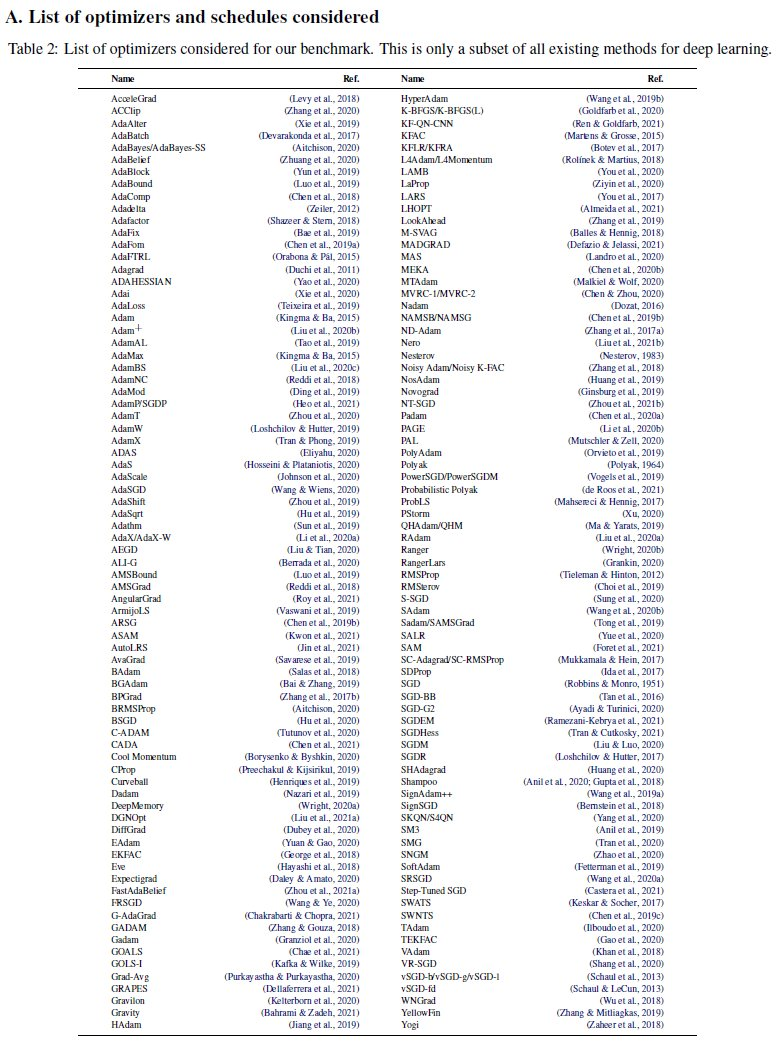
\includegraphics[width=\textwidth]{DL_optimizers}
    \end{columns}

\end{frame}
%%%%%%%%%%%%%%%%%%%%%%%%%%%%%%%%%%%%%%%%%%%%%%%%%%%%%%%%%%%%%%%%%%%%%%%%%%%%%%%


%%%%%%%%%%%%%%%%%%%%%%%%%%%%%%%%%%%%%%%%%%%%%%%%%%%%%%%%%%%%%%%%%%%%%%%%%%%%%%%
\begin{frame}{Benchmarking algorithms in practice}

Choosing the best algorithm to solve an optimization problem often depends on:\\[1em]

\begin{minipage}{.8\textwidth}
\begin{itemize}
	\item The data \mybold{scale, conditionning}
	\item The objective parameters \mybold{regularisation}
	\item The implementation \mybold{complexity, language}
\end{itemize}
\end{minipage}

\vskip2em
An impartial selection requires a time consuming {\bf benchmark}!\\[1em]


The goal of {\bf \texttt{benchopt}} is to make this step as easy as possible.

\end{frame}
%%%%%%%%%%%%%%%%%%%%%%%%%%%%%%%%%%%%%%%%%%%%%%%%%%%%%%%%%%%%%%%%%%%%%%%%%%%%%%%



%%%%%%%%%%%%%%%%%%%%%%%%%%%%%%%%%%%%%%%%%%%%%%%%%%%%%%%%%%%%%%%%%%%%%%%%%%%%%%%
\begin{frame}[fragile]{\texttt{benchopt}}

Doing a  benchmark for the $\ell_2$ regularized logistic regression with multiple solvers and datasets is now easy as calling:\\[1em]

\begin{lstlisting}[language=bash]
git clone https://github.com/benchopt/benchmark_logreg_l2
benchopt run ./benchmark_logreg_l2
\end{lstlisting}

\vskip1.5em
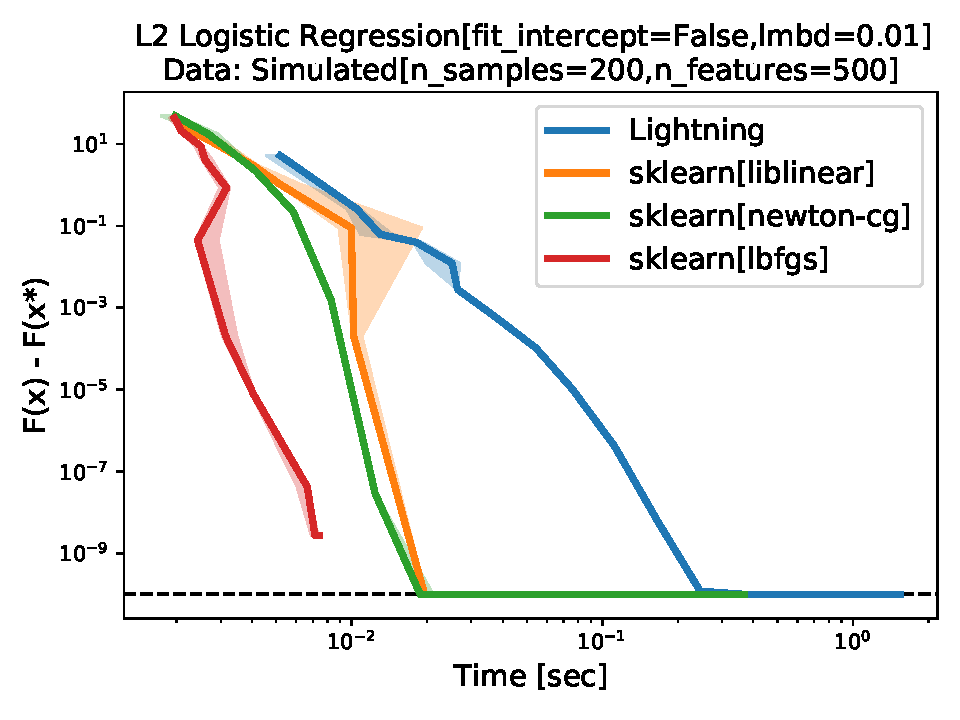
\includegraphics[width=.45\textwidth]{logreg_l2}
\hskip3ex
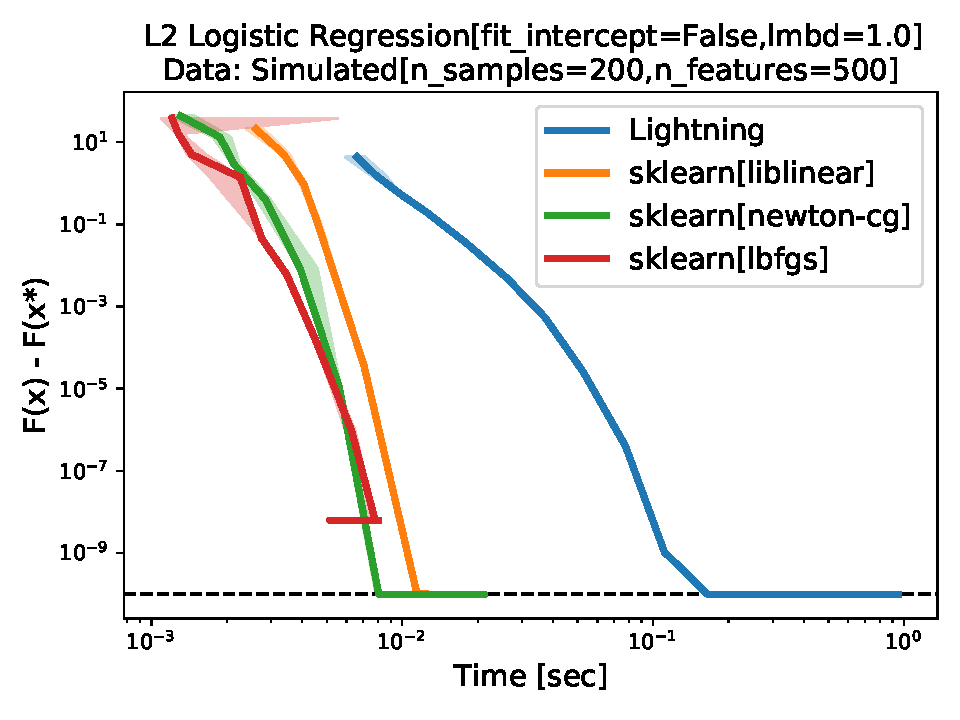
\includegraphics[width=.45\textwidth]{logreg_l2_1}

\end{frame}
%%%%%%%%%%%%%%%%%%%%%%%%%%%%%%%%%%%%%%%%%%%%%%%%%%%%%%%%%%%%%%%%%%%%%%%%%%%%%%%


%%%%%%%%%%%%%%%%%%%%%%%%%%%%%%%%%%%%%%%%%%%%%%%%%%%%%%%%%%%%%%%%%%%%%%%%%%%%%%%
\begin{frame}{\texttt{benchopt}}

    \texttt{benchopt} can also compare the same algo in different languages.\\[1em]

    Here is an example comparing PGD in: Python; R; Julia.\\[1em]
    {\centering
    \vskip.5em
    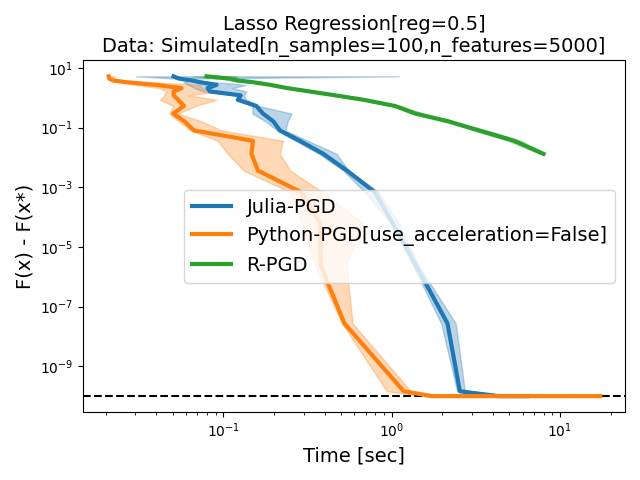
\includegraphics[width=.65\textwidth]{lasso_3_languages}\\}

\end{frame}
%%%%%%%%%%%%%%%%%%%%%%%%%%%%%%%%%%%%%%%%%%%%%%%%%%%%%%%%%%%%%%%%%%%%%%%%%%%%%%%


%%%%%%%%%%%%%%%%%%%%%%%%%%%%%%%%%%%%%%%%%%%%%%%%%%%%%%%%%%%%%%%%%%%%%%%%%%%%%%%
\begin{frame}{\texttt{benchopt}}

    \texttt{benchopt} also allow to publish easily benchmark results:\\[1em]


    {\centering

    \url{https://benchopt.github.io/results/}\\[2em]
    \vskip.5em
    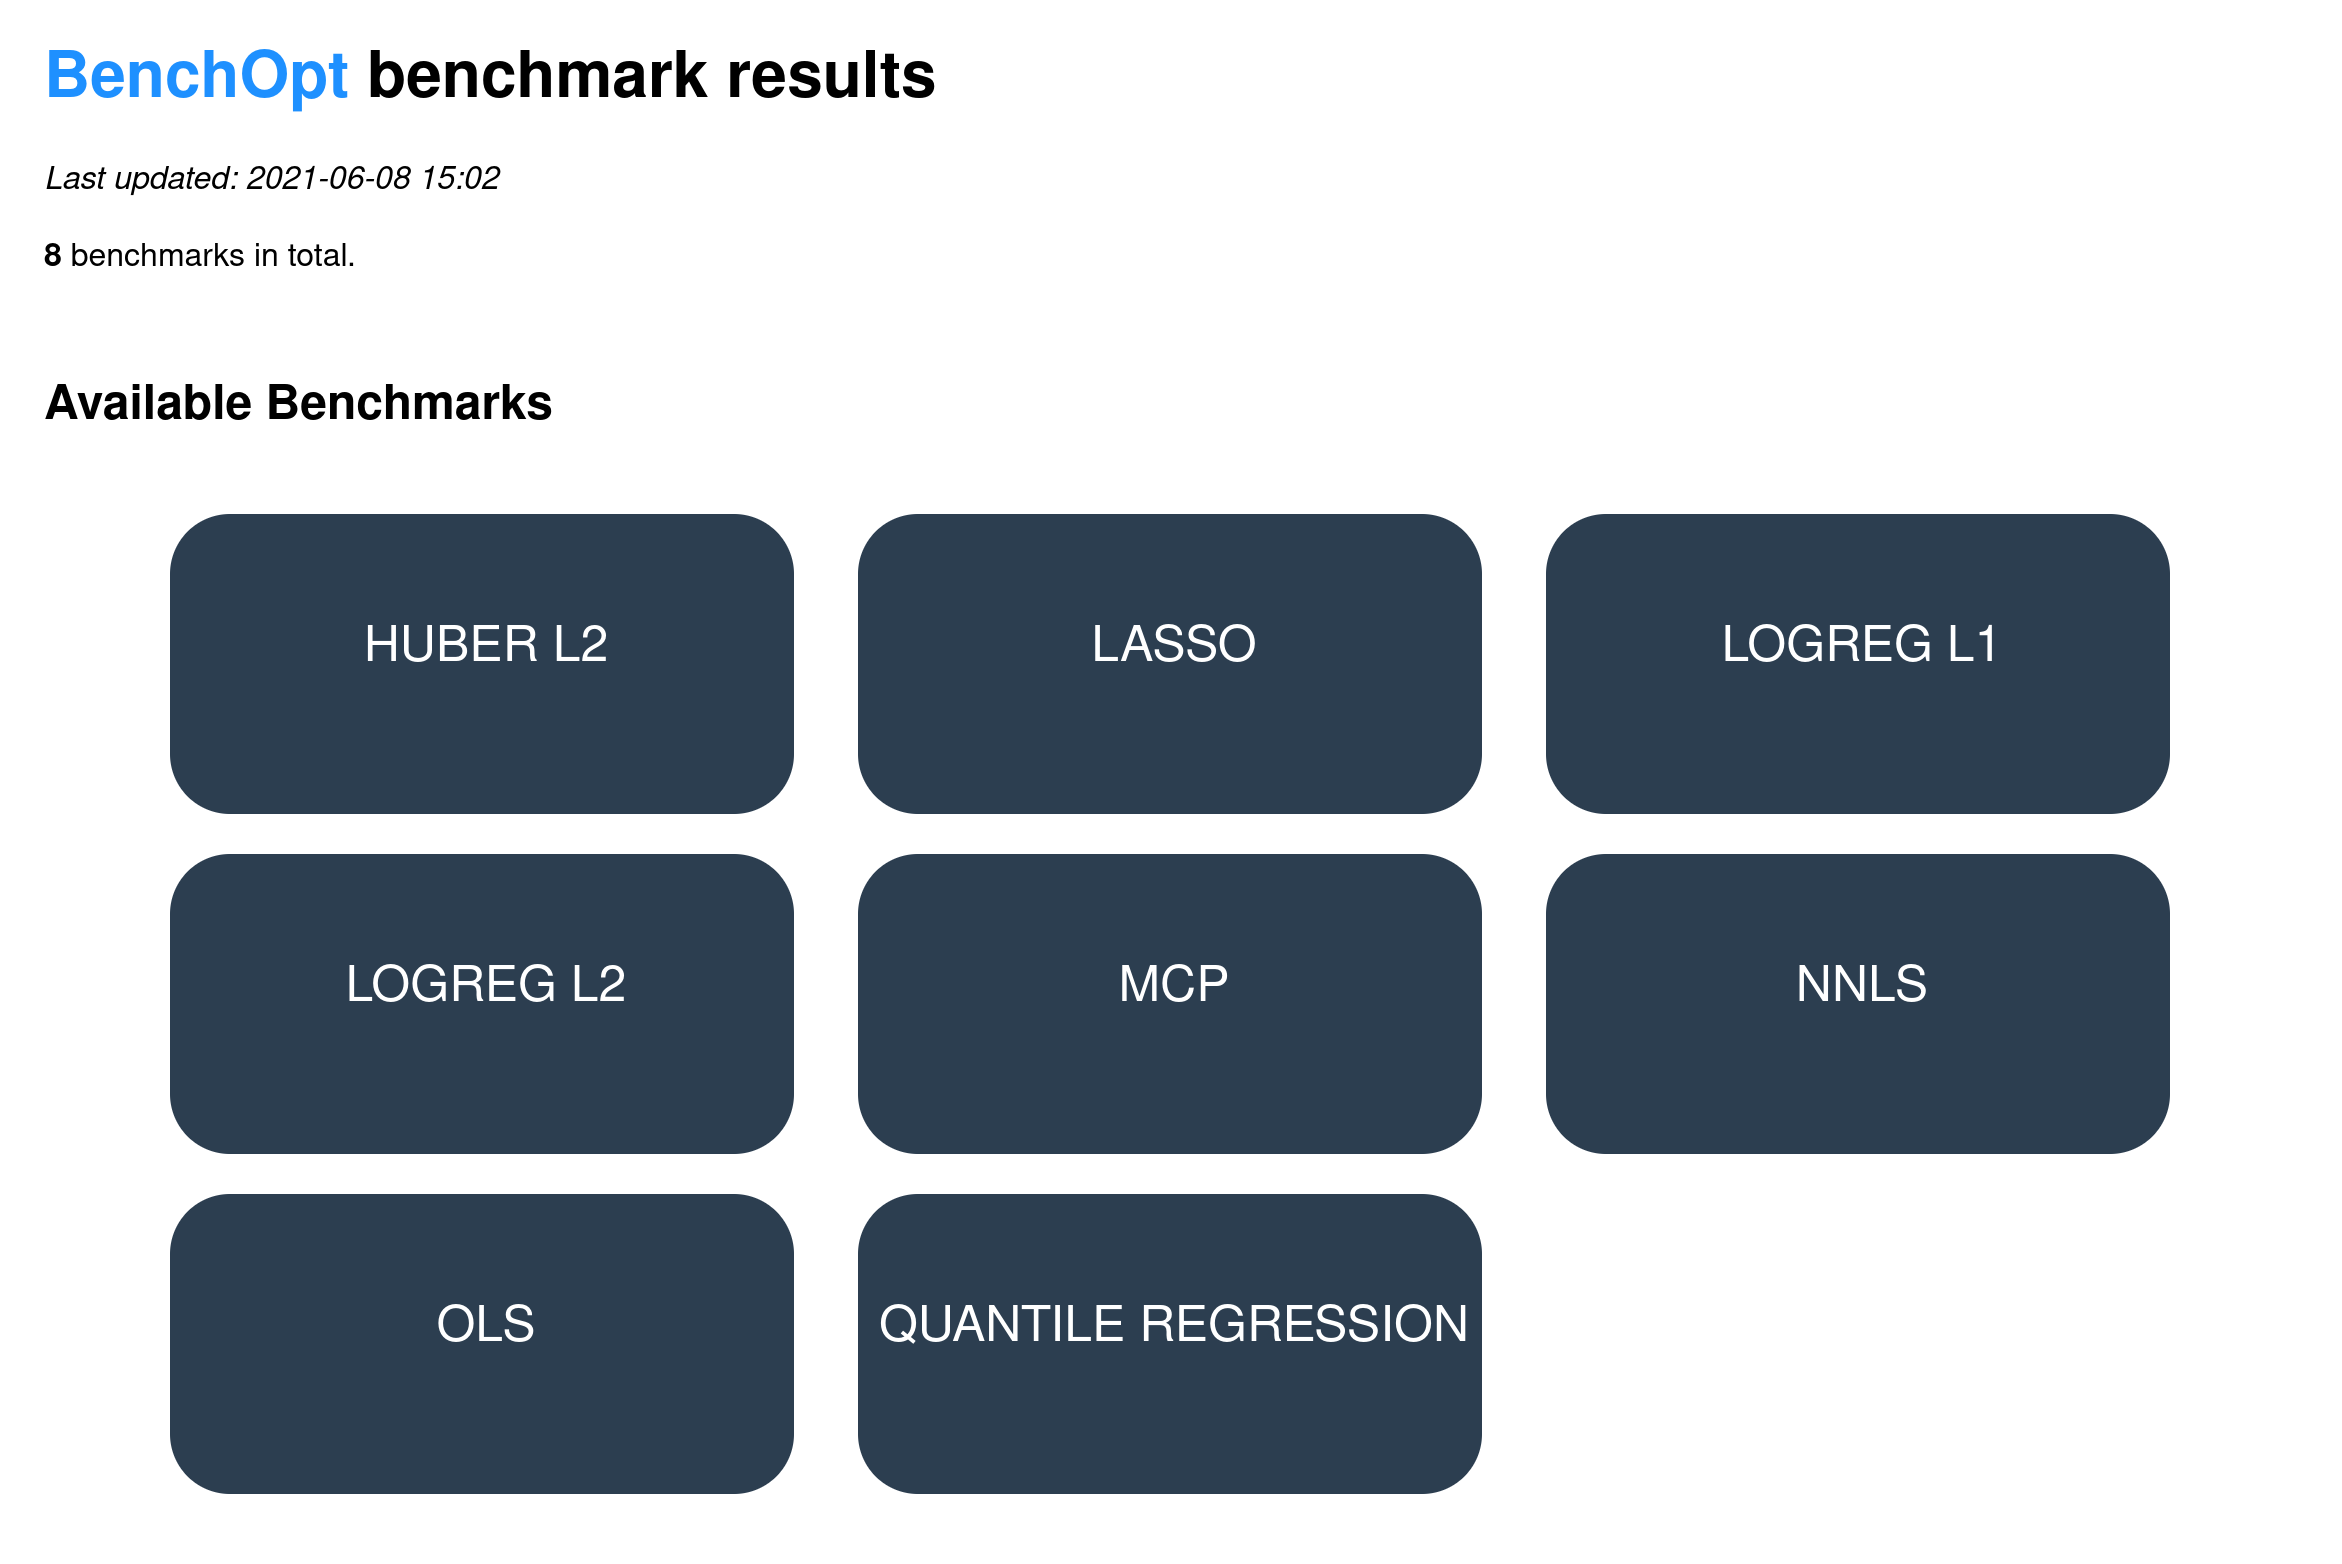
\includegraphics[width=.65\textwidth]{benchopt_results}\\}

\end{frame}
%%%%%%%%%%%%%%%%%%%%%%%%%%%%%%%%%%%%%%%%%%%%%%%%%%%%%%%%%%%%%%%%%%%%%%%%%%%%%%%


%%%%%%%%%%%%%%%%%%%%%%%%%%%%%%%%%%%%%%%%%%%%%%%%%%%%%%%%%%%%%%%%%%%%%%%%%%%%%%%
\begin{frame}{\texttt{Benchmark}}
    \centering
    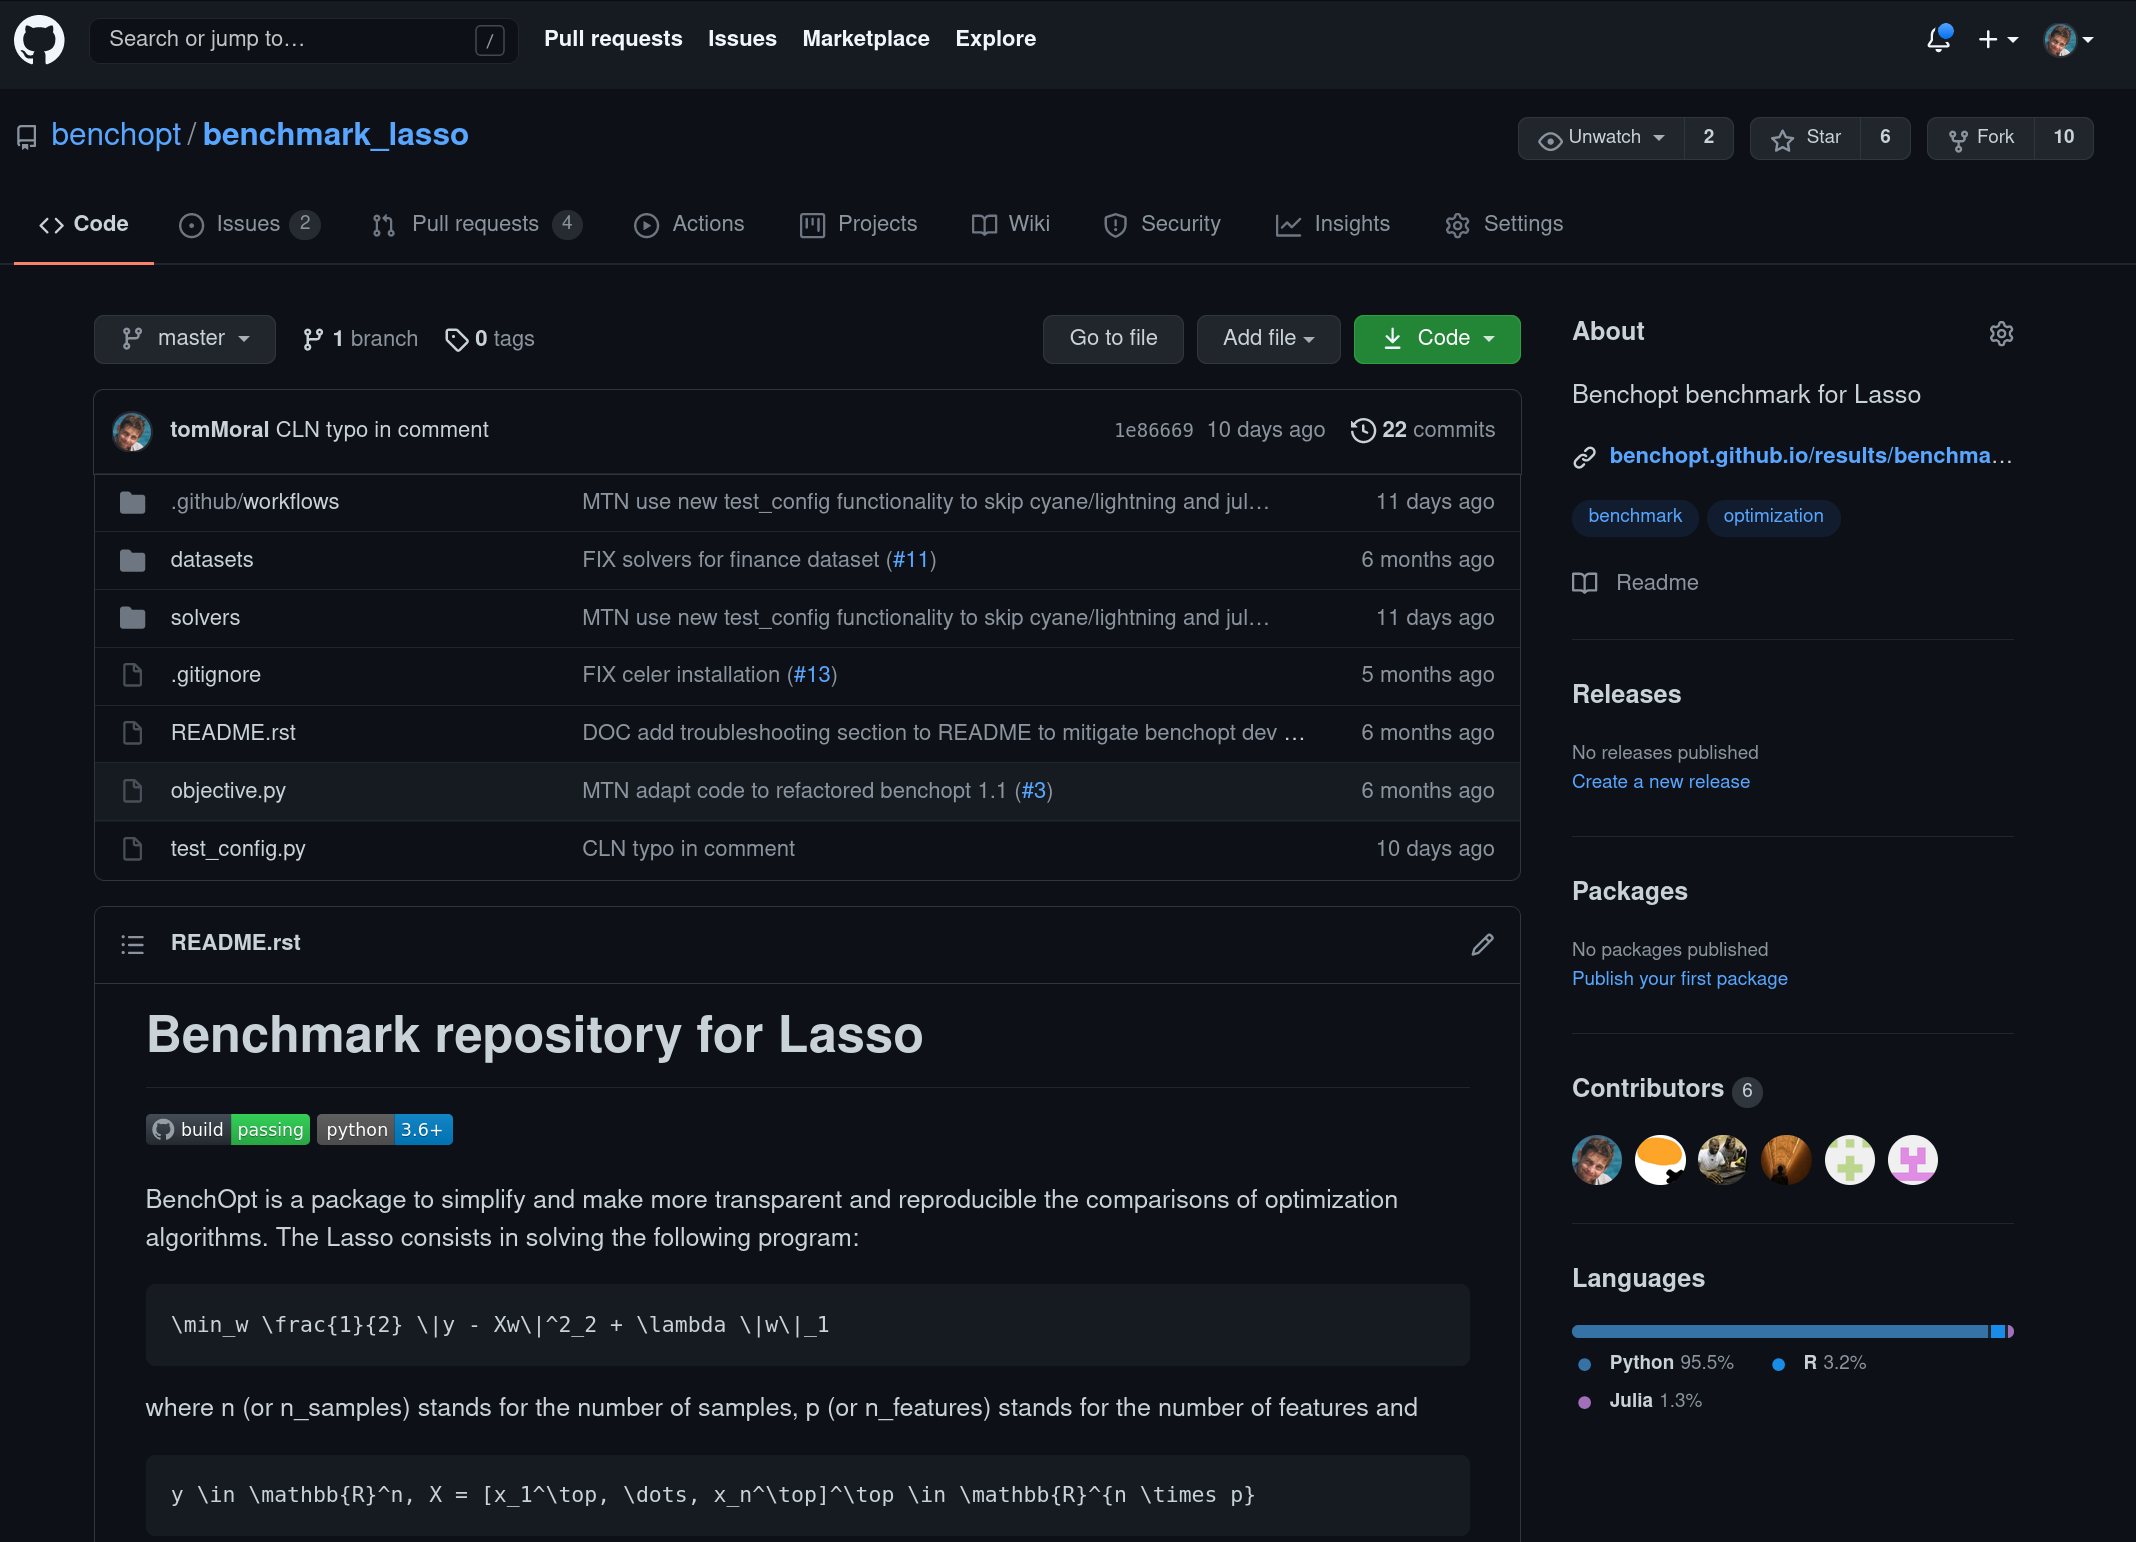
\includegraphics[width=.9\textwidth]{benchmark_lasso}\\
\end{frame}
%%%%%%%%%%%%%%%%%%%%%%%%%%%%%%%%%%%%%%%%%%%%%%%%%%%%%%%%%%%%%%%%%%%%%%%%%%%%%%%


%%%%%%%%%%%%%%%%%%%%%%%%%%%%%%%%%%%%%%%%%%%%%%%%%%%%%%%%%%%%%%%%%%%%%%%%%%%%%%%
\begin{frame}{Benchmark: principle}

A benchmark is a directory with:\\
\begin{itemize}
    \item An \lstinline+objective.py+ file with an \lstinline+Objective+
    \item A directory \lstinline+solvers+ with one file per \lstinline+Solver+
    \item A directory \lstinline+datasets+ with \lstinline+Dataset+ generators/fetchers
\end{itemize}
\vskip1em

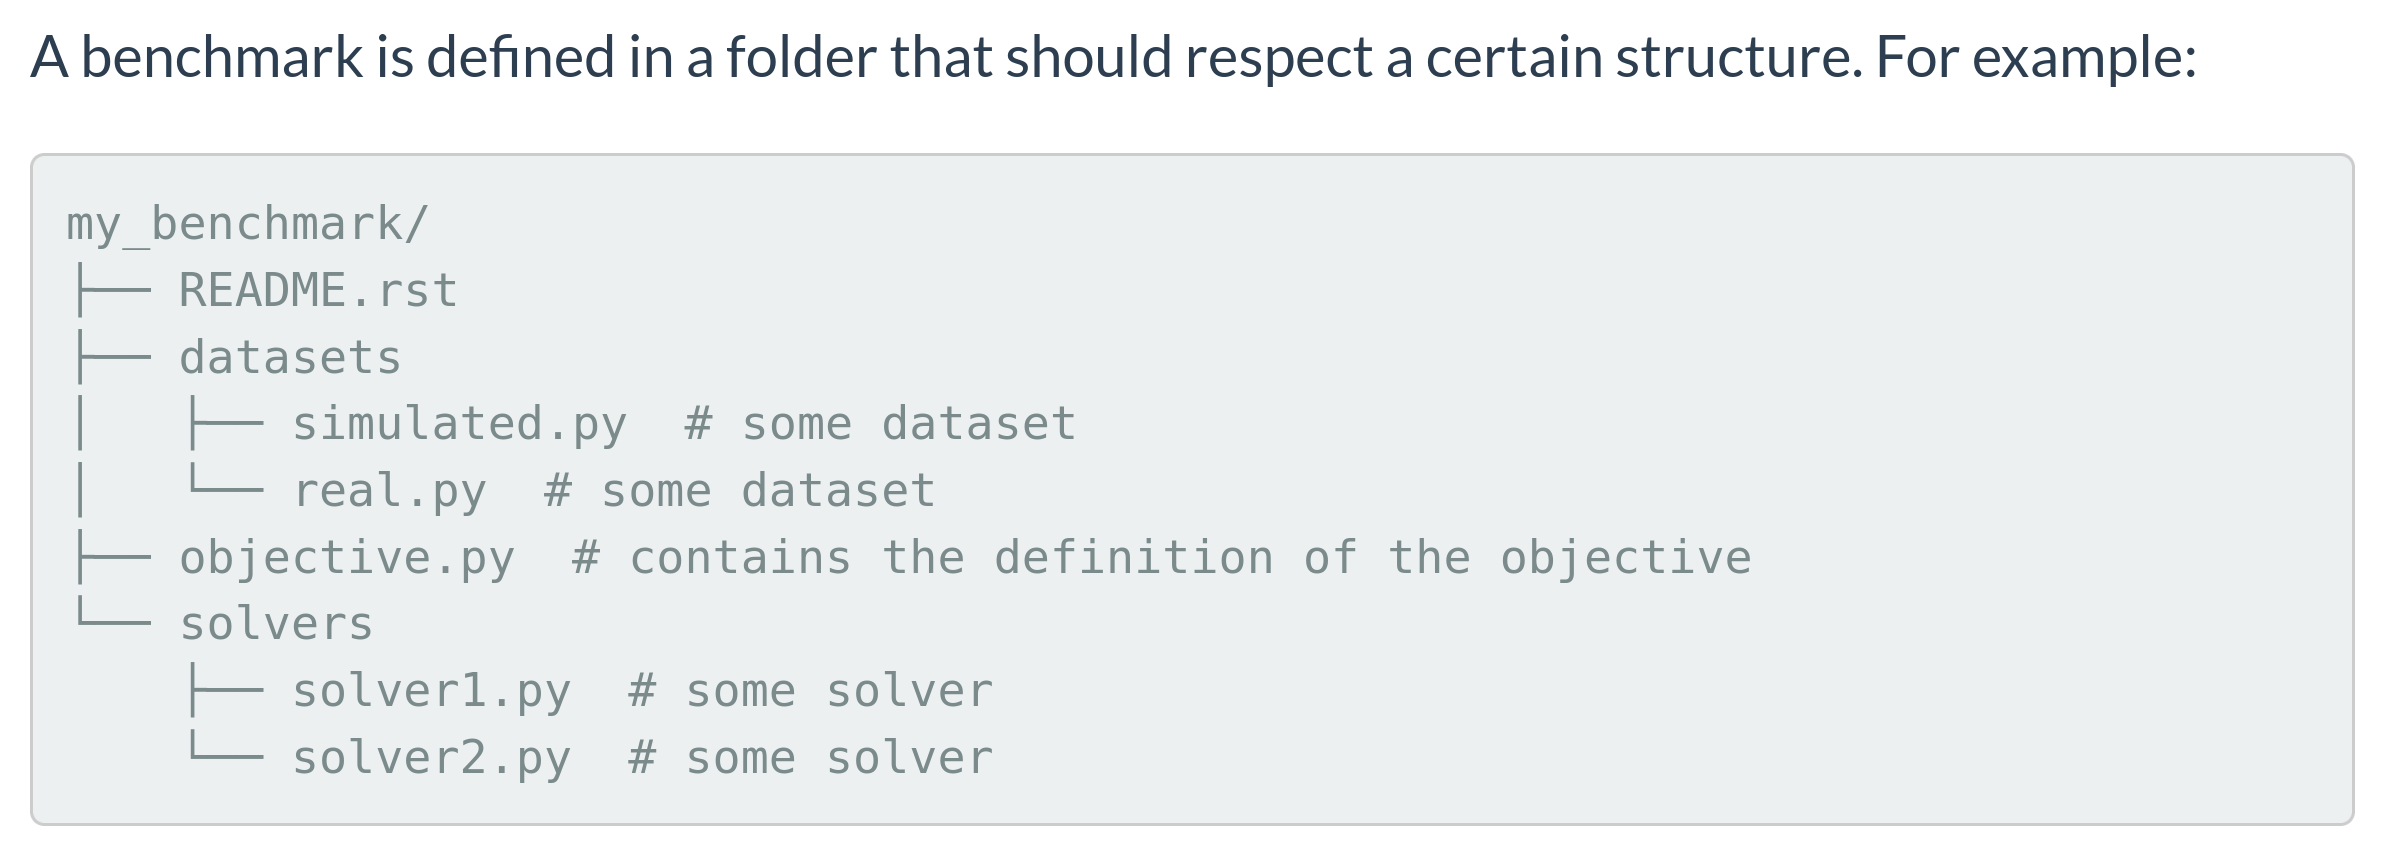
\includegraphics[width=.9\textwidth,trim={0 0 0 2.8em},clip]{benchopt_structure}

\vskip1em
The \lstinline+benchopt+ client runs a cross product and generates a csv file + convergence plots like above.
\end{frame}
%%%%%%%%%%%%%%%%%%%%%%%%%%%%%%%%%%%%%%%%%%%%%%%%%%%%%%%%%%%%%%%%%%%%%%%%%%%%%%%


%%%%%%%%%%%%%%%%%%%%%%%%%%%%%%%%%%%%%%%%%%%%%%%%%%%%%%%%%%%%%%%%%%%%%%%%%%%%%%%
\begin{frame}{Benchmark: Objective \& Dataset}

    \begin{beamercolorbox}[rounded=true,shadow=true,leftskip=2ex,colsep*=.75ex]{bgcolor}%
            \texttt{
                \textcolor{kw}{\bf class} \textcolor{var}{\bf Objective(BaseObjective)}:\\
                \hskip4ex name = \textcolor{var!60}{"Benchmark Name"}\\[1em]
                \hskip4ex\textcolor{kw}{\bf def} \textcolor{func}{set\_data}%
                (self, X, y):\\
                \hskip8ex\# Store data\\
                \hskip4ex\textcolor{kw}{\bf def} \textcolor{func}{compute}%
                (self, beta):\\
                \hskip8ex return dict\{obj1:.., obj2:..\}\\
                \hskip4ex\textcolor{kw}{\bf def} \textcolor{func}{to\_dict}%
                (self):\\
                \hskip8ex return dict\{X:.., y:.., reg:..\}\\
            }
    \end{beamercolorbox}%
    \vskip1.5em
    \begin{beamercolorbox}[rounded=true,shadow=true,leftskip=2ex,colsep*=.75ex]{bgcolor}%
        \texttt{
            \textcolor{kw}{\bf class} \textcolor{var}{\bf Dataset(BaseDataset)}:\\
            \hskip4ex name = \textcolor{var!60}{"Dataset Name"}\\[1em]
            \hskip4ex\textcolor{kw}{\bf def} \textcolor{func}{get\_data}%
            (self):\\
            \hskip8ex return dict\{X:.., y:..\}\\
        }
    \end{beamercolorbox}%

\end{frame}
%%%%%%%%%%%%%%%%%%%%%%%%%%%%%%%%%%%%%%%%%%%%%%%%%%%%%%%%%%%%%%%%%%%%%%%%%%%%%%%


%%%%%%%%%%%%%%%%%%%%%%%%%%%%%%%%%%%%%%%%%%%%%%%%%%%%%%%%%%%%%%%%%%%%%%%%%%%%%%%
\begin{frame}{Benchmark: Solver}

    \begin{beamercolorbox}[rounded=true,shadow=true,leftskip=2ex,colsep*=.75ex]{bgcolor}%
        \texttt{
            \textcolor{kw}{\bf class} \textcolor{var}{\bf Solver(BaseSolver)}:\\
            \hskip4ex name = \textcolor{var!60}{"Solver Name"}\\[1em]
            \hskip4ex\textcolor{kw}{\bf def} \textcolor{func}{set\_objective}%
            (self, X, y, reg):\\
            \hskip8ex\# Store objective info\\[1em]
            \hskip4ex\textcolor{kw}{\bf def} \textcolor{func}{run}%
            (self, n\_iter):\\
            \hskip8ex \# Run computations for \textcolor{var}{n\_iter}\\[1em]
            \hskip4ex\textcolor{kw}{\bf def} \textcolor{func}{get\_result}%
            (self):\\
            \hskip8ex return \textcolor{var}{beta}\\
        }
    \end{beamercolorbox}%

    \vskip1em
    \rem {\bf Flexible API}\\
    \begin{itemize}
        \item \texttt{\textcolor{func}{get\_data}} and \texttt{\textcolor{func}{set\_objective}} allow to compatibility between packages.
        \item \texttt{\textcolor{var}{n\_iter}} can be replaced with a tolerance or a callback.
    \end{itemize}

\end{frame}
%%%%%%%%%%%%%%%%%%%%%%%%%%%%%%%%%%%%%%%%%%%%%%%%%%%%%%%%%%%%%%%%%%%%%%%%%%%%%%%



%%%%%%%%%%%%%%%%%%%%%%%%%%%%%%%%%%%%%%%%%%%%%%%%%%%%%%%%%%%%%%%%%%%%%%%%%%%%%%%
\begin{frame}{\texttt{benchopt}}
    \centering
    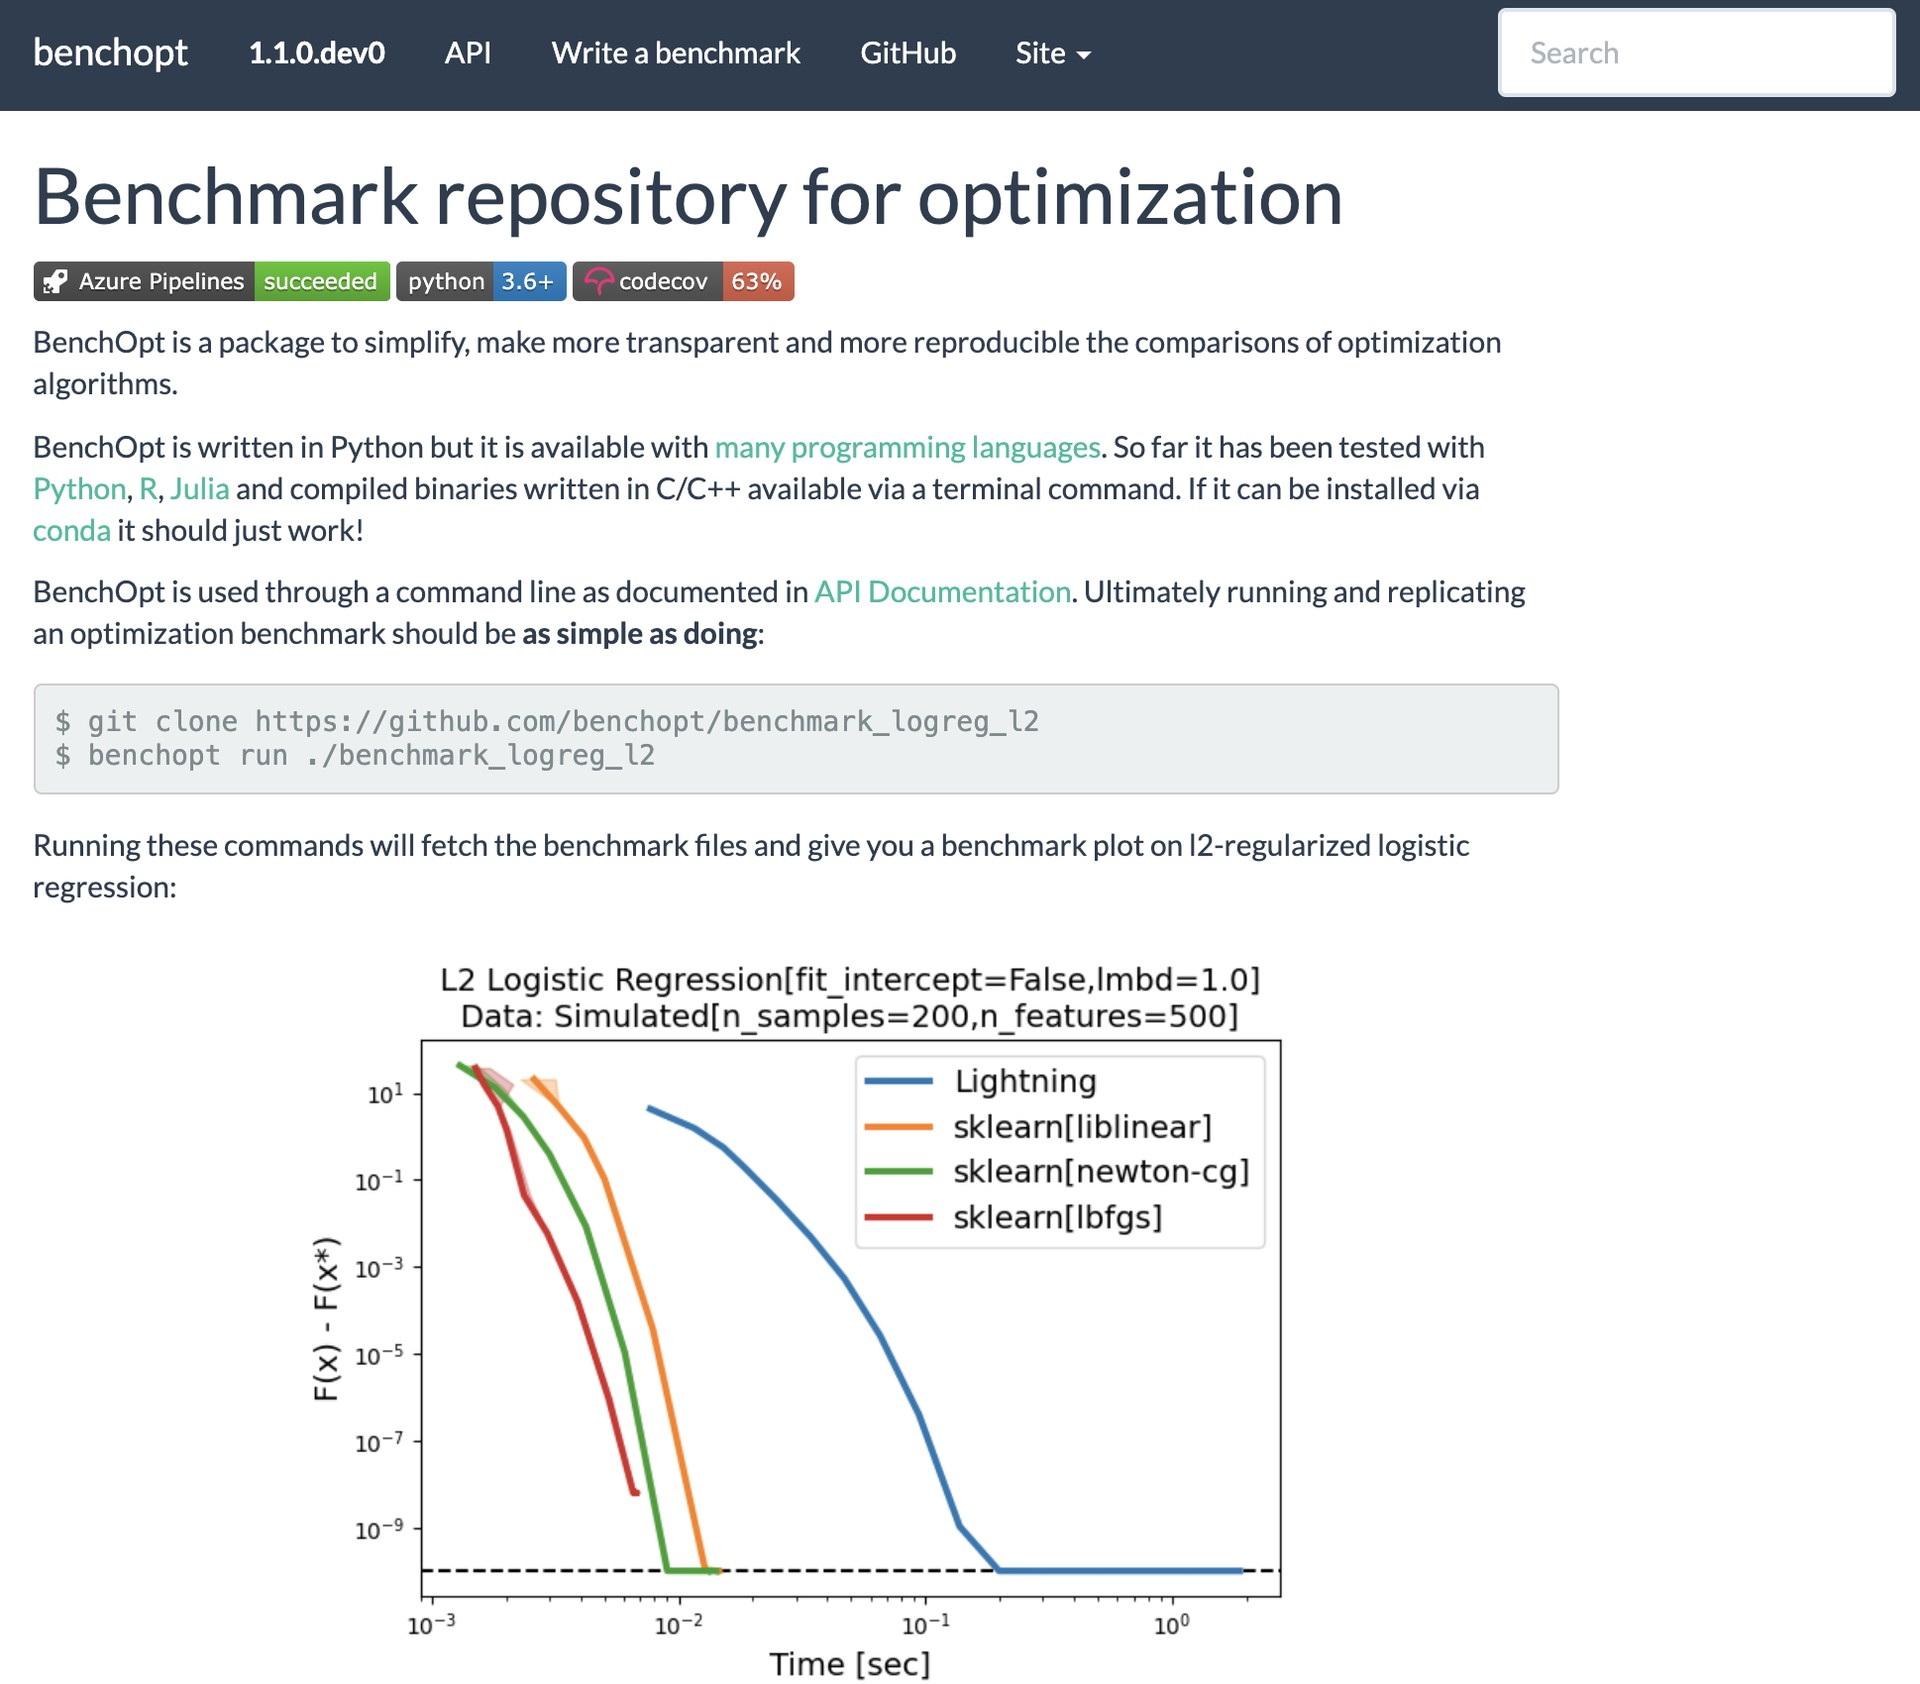
\includegraphics[width=.9\textwidth]{benchopt}\\
\end{frame}
%%%%%%%%%%%%%%%%%%%%%%%%%%%%%%%%%%%%%%%%%%%%%%%%%%%%%%%%%%%%%%%%%%%%%%%%%%%%%%%



%%%%%%%%%%%%%%%%%%%%%%%%%%%%%%%%%%%%%%%%%%%%%%%%%%%%%%%%%%%%%%%%%%%%%%%%%%%%%%%
\begin{frame}{\texttt{benchopt: Making tedious tasks easy}}

    {\bf Automatizing tasks:}\\[1.2em]
    \begin{itemize}\itemsep.7em
        \item Automatic installation of competitors solvers.
        \item Parametrized datasets, objectives and solvers and run on cross products.
        \item Make sure to quantify the variance.
        \item Automatic caching.
        \item First visualization of the results.
        \item Automatic parallelization, ... ?
    \end{itemize}
\end{frame}
%%%%%%%%%%%%%%%%%%%%%%%%%%%%%%%%%%%%%%%%%%%%%%%%%%%%%%%%%%%%%%%%%%%%%%%%%%%%%%%



%%%%%%%%%%%%%%%%%%%%%%%%%%%%%%%%%%%%%%%%%%%%%%%%%%%%%%%%%%%%%%%%%%%%%%%%%%%%%%%
\begin{frame}{Credits}
    \begin{figure}
         \centering
         \hfill
         \begin{subfigure}[b]{0.188\textwidth}
             \centering
            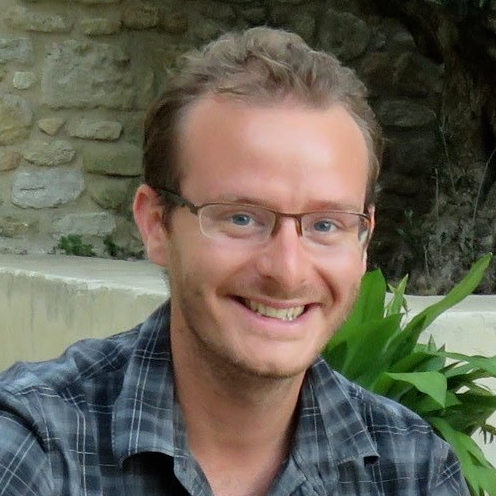
\includegraphics[width=0.969\textwidth]{jsalmon}
            \caption{J. Salmon\\ INRIA Parietal}
         \end{subfigure}
         \hfill
         \begin{subfigure}[b]{0.188\textwidth}
             \centering
            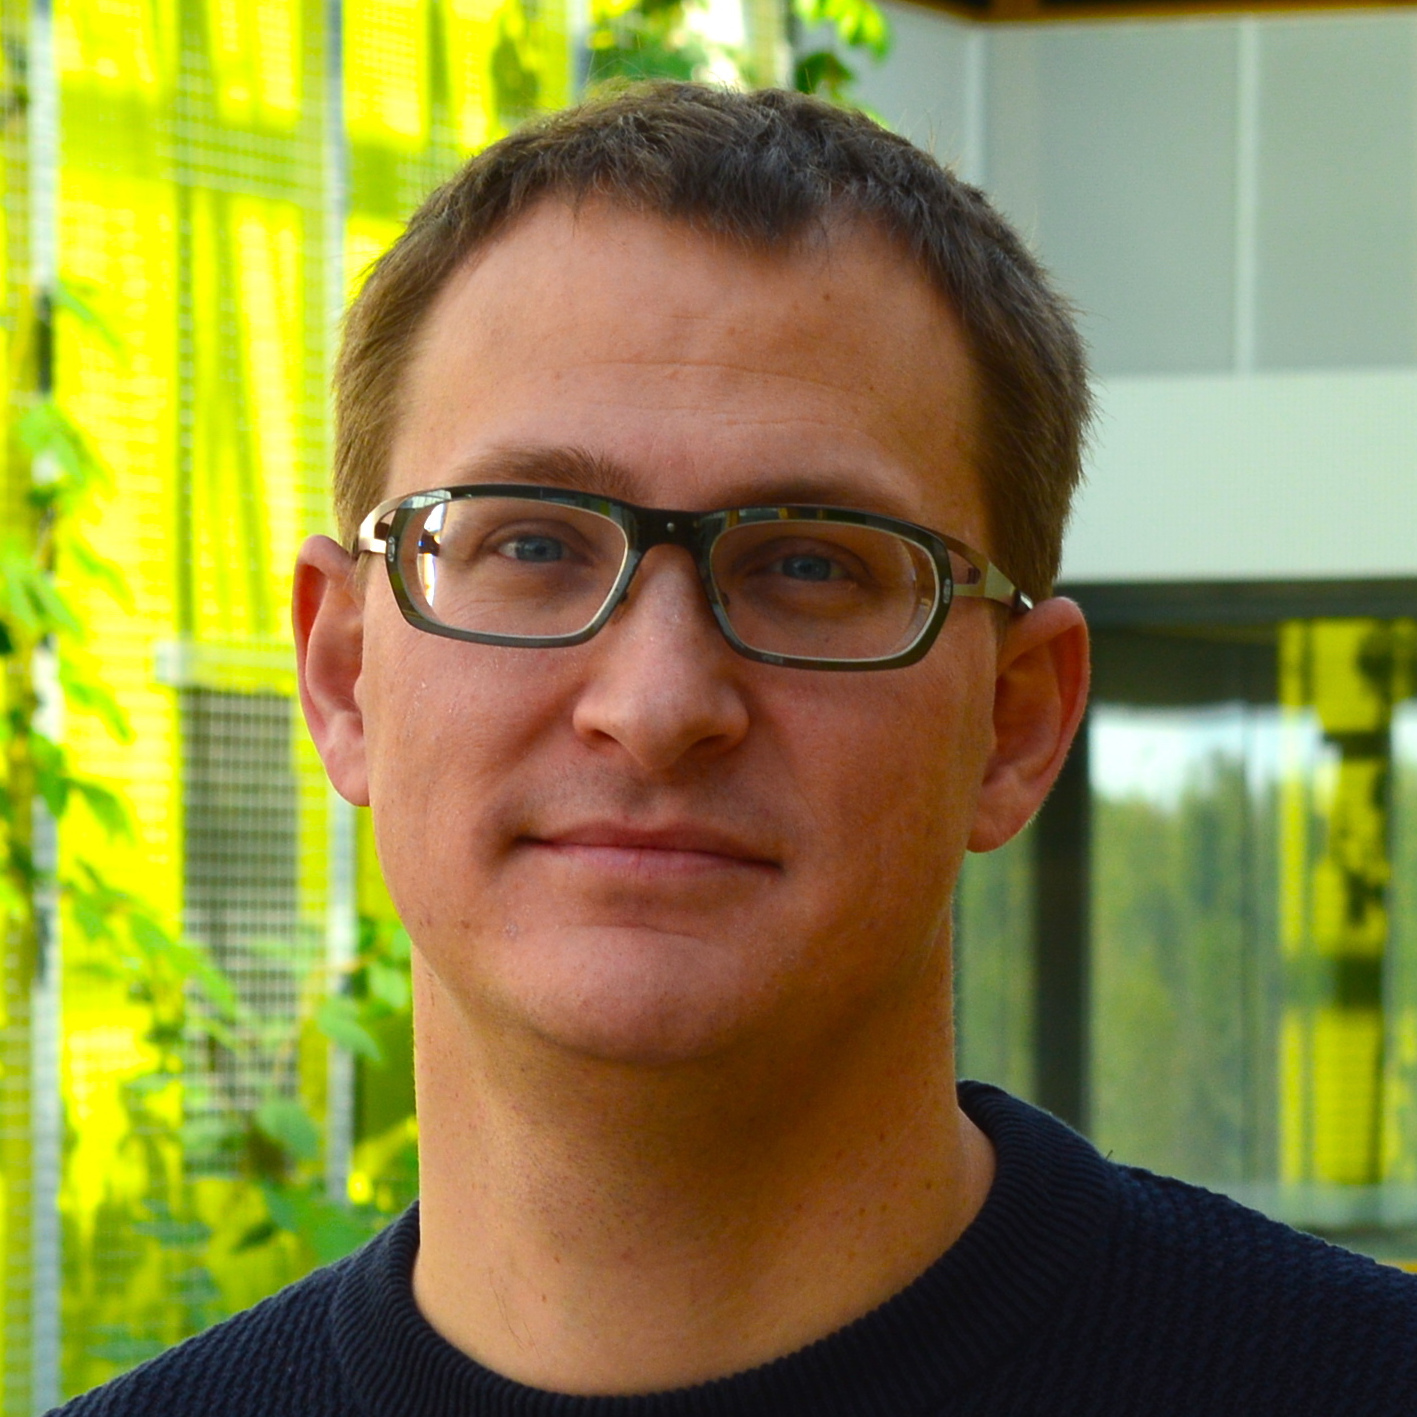
\includegraphics[width=0.969\textwidth]{agramfort}
            \caption{A. Gramfort\\ INRIA Parietal}
         \end{subfigure}
         \hfill
         \begin{subfigure}[b]{0.188\textwidth}
             \centering
            
\includegraphics[width=0.969\textwidth]{tommoral}
            \caption{T. Moreau\\ INRIA Parietal}
         \end{subfigure}\hfill\\[2em]
         \begin{subfigure}[b]{0.188\textwidth}
             \centering
             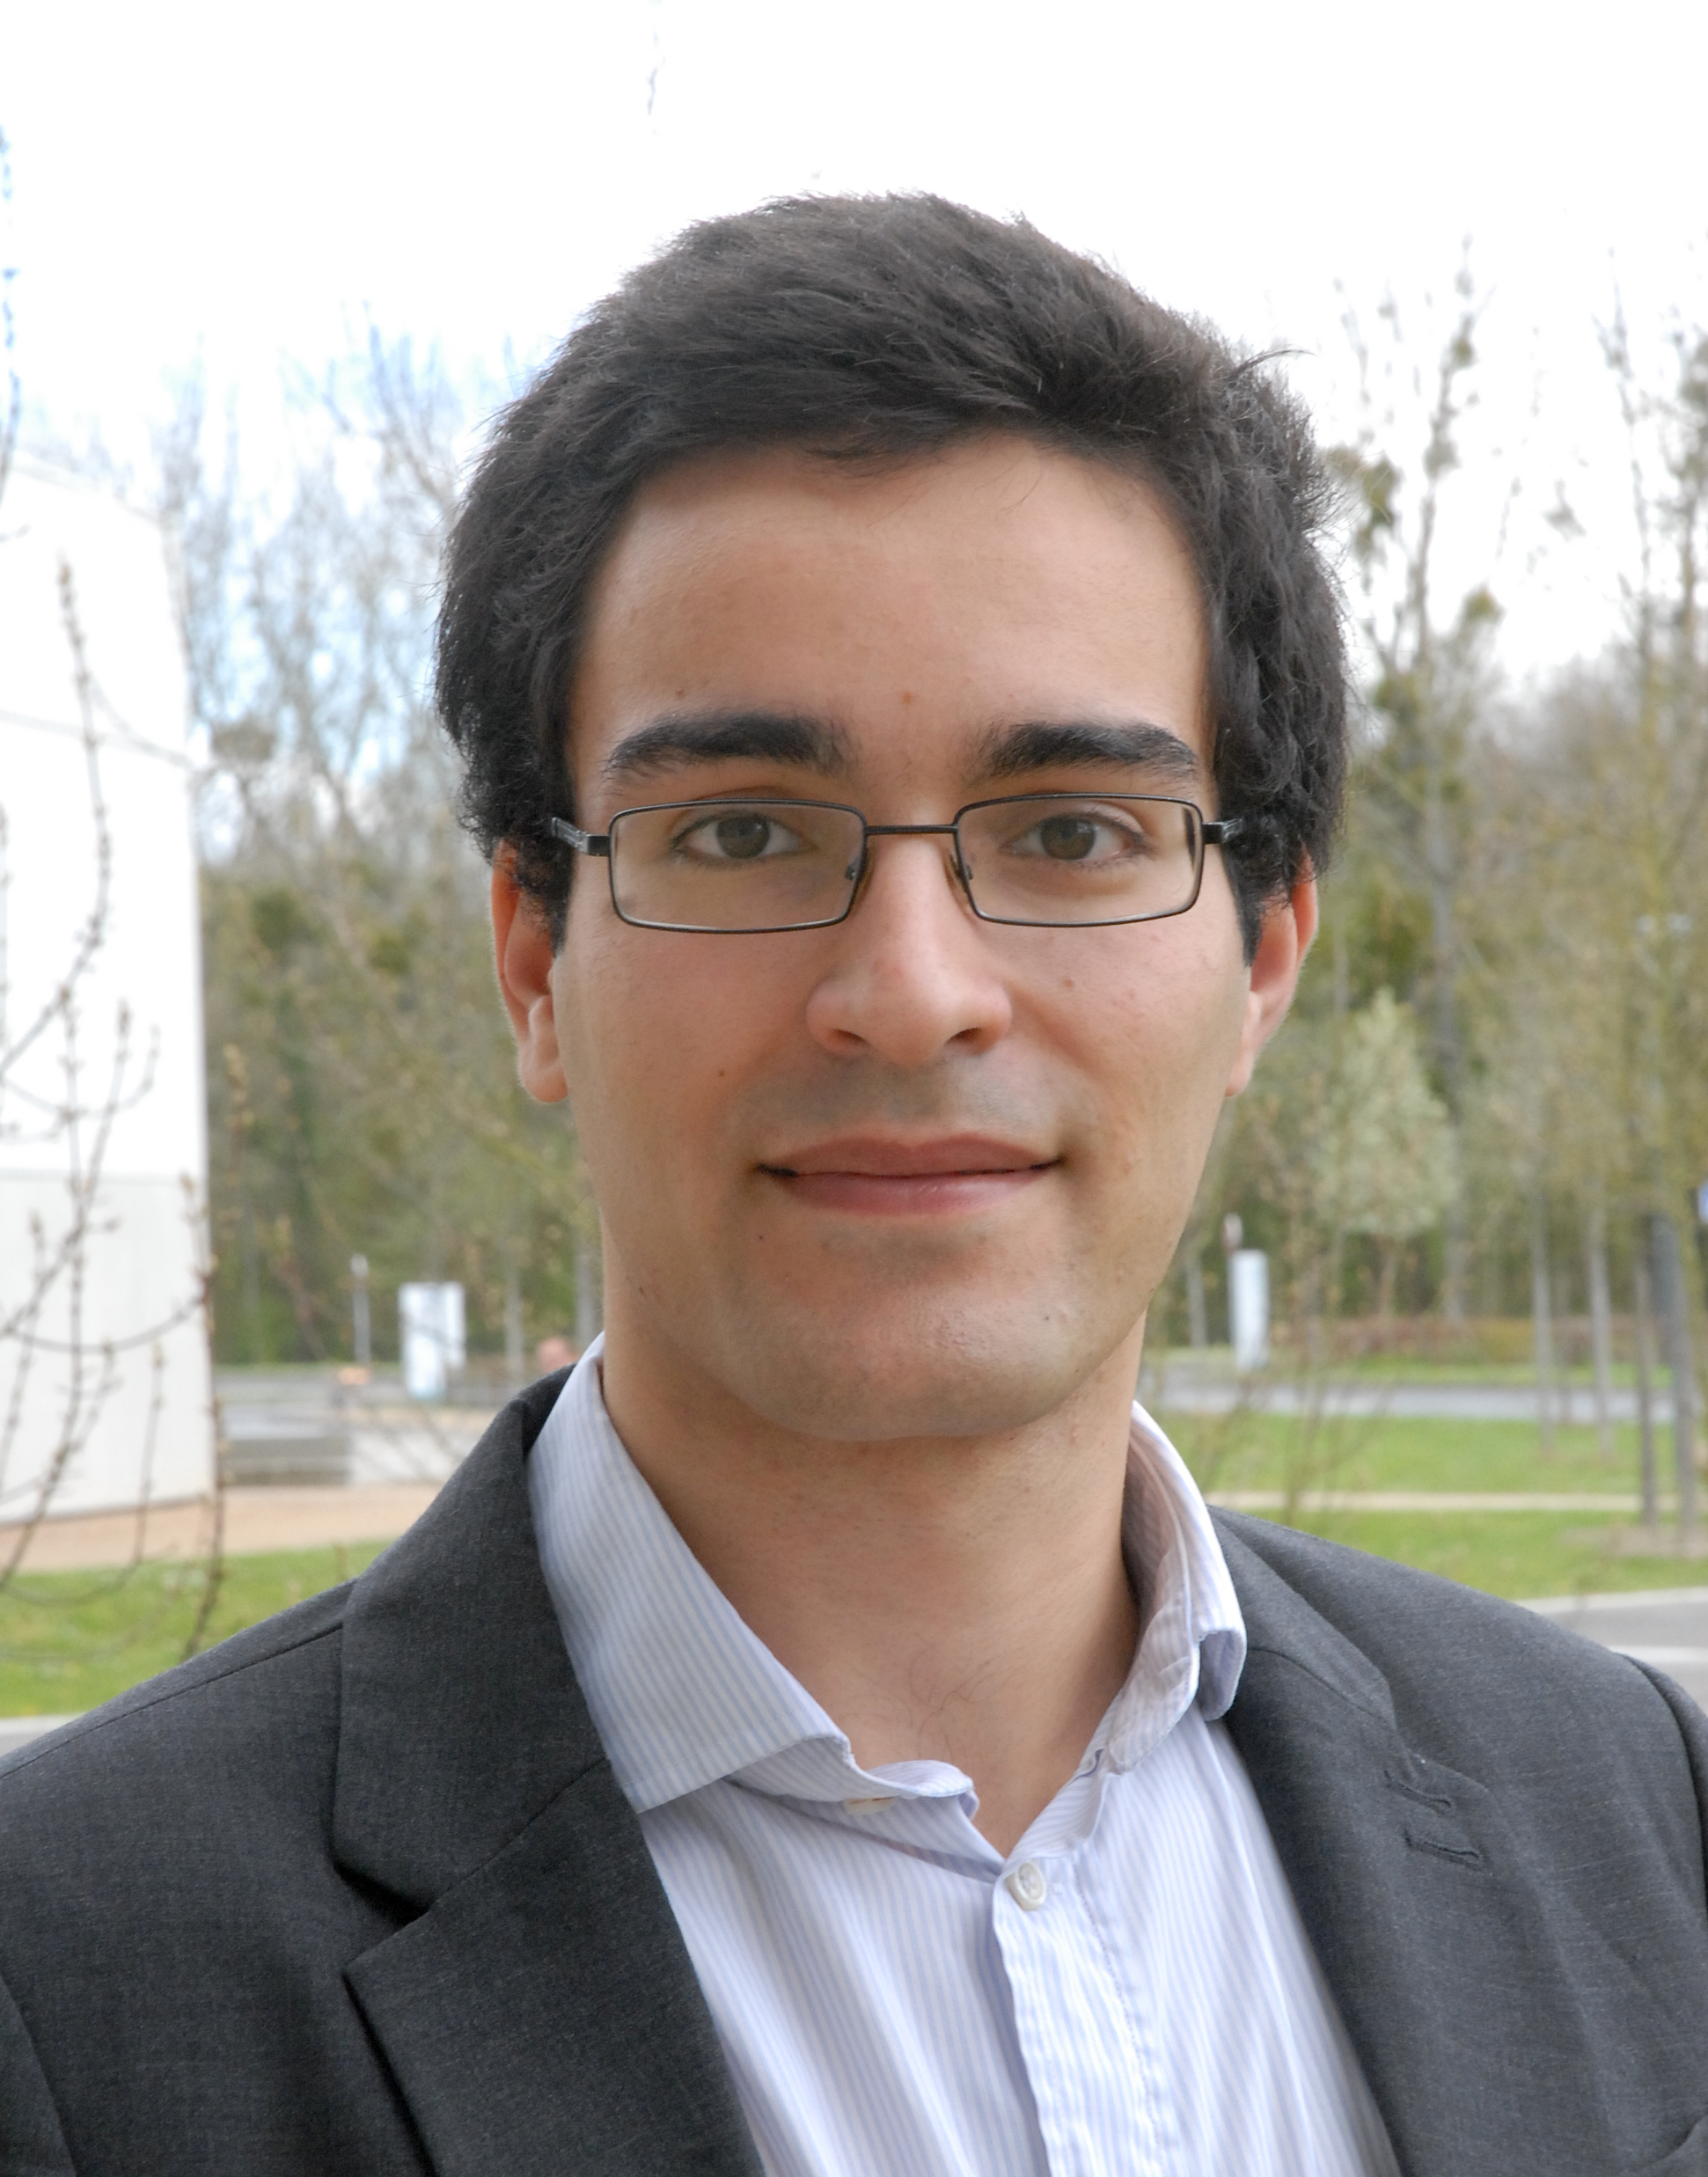
\includegraphics[width=0.969\textwidth]{nidham}
             \caption{N. Gazagnadou\\Telecom Paris}
         \end{subfigure}
         \hfill
         \begin{subfigure}[b]{0.188\textwidth}
             \centering
            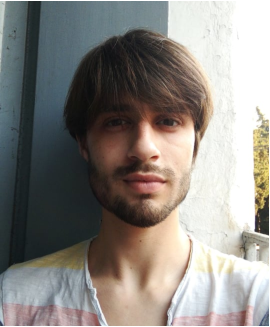
\includegraphics[width=0.969\textwidth]{tanglef}
             \caption{T. Lefort\\Univ. Montpellier}
         \end{subfigure}
         \hfill
         \begin{subfigure}[b]{0.188\textwidth}
             \centering
             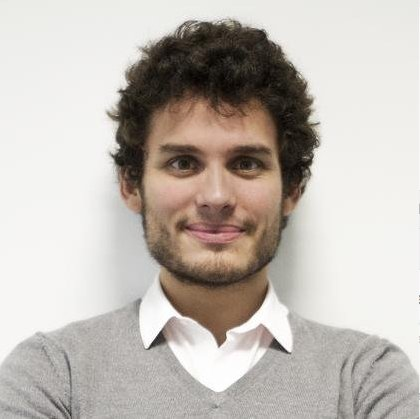
\includegraphics[width=0.969\textwidth]{mmassias}
             \caption{M. Massias\\Univ. of Genova }
         \end{subfigure}
         \hfill
         \begin{subfigure}[b]{0.188\textwidth}
             \centering
            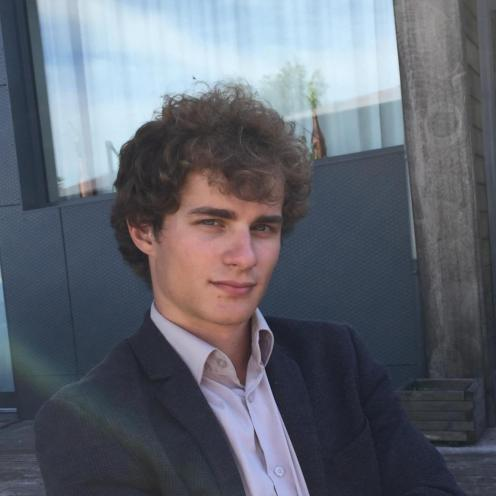
\includegraphics[width=0.969\textwidth]{tomdlt}
            \caption{T. Dupré la Tour\\ UC Berkeley}
         \end{subfigure}
    \end{figure}
\end{frame}
%%%%%%%%%%%%%%%%%%%%%%%%%%%%%%%%%%%%%%%%%%%%%%%%%%%%%%%%%%%%%%%%%%%%%%%%%%%%%%%




% %%%%%%%%%%%%%%%%%%%%%%%%%%%%%%%%%%%%%%%%%%%%%%%%%%%%%%%%%%%%%%%%%%%%%%%%%%%%%%%
% % Uncomment for references
% \begin{frame}{Bibliographie}
% \printbibliography
% \end{frame}
%  %%%%%%%%%%%%%%%%%%%%%%%%%%%%%%%%%%%%%%%%%%%%%%%%%%%%%%%%%%%%%%%%%%%%%%%%%%%%%%



\end{document}
